\chapter{Context and Dependency Injection}
 
\section{Inversion of Control}
\label{sec:ioc}

Inversion of Control (IoC) ist ein Paradigma das in der objektorientierten Programmierung verwendet wird.  Oft wird in diesem Zusammenhang das Hollywood-Prinzip (\emph{Don't call us, we'll call you}) verwendet, weil diesen Satz oft Schauspielamateure zu hören kriegen. In der klassischen Programmierung ruft der selbst programmierte (oder spezifische) Code den wiederverwendbaren Code auf (z.B. eine Funktion in einem Framework). Bei IoC wird dieser Vorgang umgekehrt. Das Framework (z.B. CDI) ruft den eignen Code auf und befreit den Programmierer dadurch von der Initialisierung der ganzen Komponenten (Hast du jemals eine \verb|main()|-Methode in Java EE gesehen?). Dadurch kann das Programm besser modularisiert und erweitert (keine Seiteneffekte) werden. Es gibt folgende Pattern um das IoC Paradigma umzusetzen:
\begin{itemize}
	\item Factory
	\item Service Locator
	\item Dependency Injection
	\item Template
	\item Strategy
\end{itemize}
Wie man sieht ist IoC ein sehr breit gefächerter Begriff. Abbildung \ref{fig:service-locator-di} zeigt das Service Locator und Dependency Injection Pattern. Diese Patterns übernehmen die Kontrolle wie man eine Applikation zusammensteckt. Beim Service Locator fragt \verb|ClassA| den Service Locator explizit nach Instanzen der Abhängikeiten. Beim DI gibt es keine expilzite Anfrage der \verb|ClassA|.

\begin{figure}
\centering
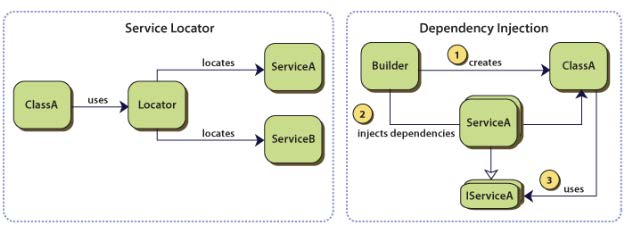
\includegraphics[width=0.7\linewidth]{fig/service-locator-di}
\caption{Service Locator / Dependency Injection}
\label{fig:service-locator-di}
\end{figure}

\section{CDI}

CDI besteht grundsätzlich aus folgenden zwei Funktionen:
\begin{description}
	\item[Context:] Komponenten werden an einen definierte aber erweiterbaren Life Cycle gebunden.
	\item[Dependency Injection:] Komponenten können typensicher in andere injected werden. Dabei kann beim Deployment entschieden werden, welche Implementation für ein Interface verwendet werden soll.
\end{description}
Zusätzlich zu den oben aufgeführten Basis-Funktionen bietet es noch folgende an:
\begin{itemize}
	\item Mit Interceptoren können Querschnittfunktionen (z.B. Logging) einfach implementiert werden. Mit CDI lässt sich ein Interceptor typensicher (\textbf{strong typing}) mit der entsprechenden Komponente verbinden.
	\item Objekte können über Events interagieren
	\item Über ein Service Provider Interface (SPI) können externe Frameworks sauber in Java EE integriert werden.
\end{itemize}
All diese Funktionen dienen einer \textbf{losen Kopplung} zwischen Komponenten. Konkret wird die Implementation von der Schnittelle einer Komponente getrennt. Dadurch müssen folgende Fragen nicht mehr gestellt werden:
\begin{itemize}
	\item Wo soll ich die Referenz aufbewahren wenn ich es momentan nicht verwende?
	\item Gibt es eine alternative Implementationsmöglichkeit, so dass die Implementation vom Deployment abhängig ist?
	\item Wie soll ich dieses Objekt sharen zwischen anderen Objekten?
\end{itemize}
Zudem wird muss der Programmierer auch nicht um den Life Cycle der Komponenten kümmern. Dadurch fallen folgende Fragen weg:
\begin{itemize}
	\item Was ist der Lebenszyklus dieses Objektes?
	\item Wie viele simultane Clients kann es haben?
	\item Ist es multithreaded?
	\item Muss ich es explizit zerstören?
\end{itemize}

\section{Bean}

Ein Objekt dessen Life Cycle vom Container gesteuert wird ist ein Bean. CDI unterstützt managed Beans (wird von JSF verwendet) und EJB Session Beans (wird für Business Logic verwendet). Mit Java EE 6 wurde aber ein neues Konzept für Beans eingeführt, welches mit den oberen nichts zu tun hat. In CDI muss ein Bean folgende Eigenschaften haben:
\begin{itemize}
	\item ein (nicht leeres) Set von Bean Typen
	\item ein (nicht leeres) Set von Qualifiers
	\item ein Scope
	\item Optional, ein Bean EL (Expression Language) Name
	\item Ein Set von Interceptor Bindings
	\item Eine Bean Implementaion
\end{itemize}
In ein Bean kann dann mit \verb|@Inject| fast alles injected werden (z.B. POJO, Session Beans, Persistence Context). 

Jede Bean in CDI hat einen Scope. Der Scope definiert Lebenszyklus und Sichtbarkeit einer Bean Instanz (siehe Abschnitt \ref{sec:scope}). Wenn eine Bean keinen expliziten Scope hat (z.B. EJB Bean) weisst CDI einen Pseudo-Scope zu. Es lassen sich mit CDI auch eigene Scopes erstellen.

Möchte man Beans in nicht Java Code verwenden (z.B. in JSF) muss man ihm einen EL-Namen zuweisen. Mit der Annotation \verb|@Named("cart")| wird dem Bean einen EL-Namen zugewiesen und es kann z.B. in JSF verwendet werden (\verb|#{cart.lineItems}|).

\section{Bean Typen \& Qualifiers}

CDI steckt seine Kompontenten aufgrund der Bean Typen und Qualifiers zusammen. Ein Bean Typ ist eine Klasse oder ein Interface, welches für den Client sichtbar ist. Listing \ref{lst:bean-typen} zeigt zwei Beispiele.
\begin{lstlisting}[caption=Bean Typen, label=lst:bean-typen]
// Hat die Typen BookShop, Business, Shop und java.lang.Object
public class BookShop extends Business implements Shop<Book> {...}

// Hat nur die Typen BookShop, Auditabele und java.lang.Object aber nicht 
// BookShopBean, weil dieser für den Client nicht sichtbar ist.
@Stateful
public class BookShopBean extends BookShop implements Auditable {...}

// Mit @Typed lässt sich der Bean Typ beschränken. Diese Bean hat nur den Typ Shop 
// und java.lang.Object
@Typed(Shop.class)
public class BookShop extends Business implements Shop<Book> {...}
\end{lstlisting}
Mit Qualifiers lassen sich typensicher verschiedene Implementation einer Schnittstelle per Annotation auswählen. Listing \ref{lst:qualifier} zeigt wie ein Qualifier definiert wird.
\begin{lstlisting}[caption=Qualifier, label=lst:qualifier]
// Annotation mit @Qualifier erstellen
@Qualifier
@Target({TYPE, METHOD, PARAMETER, FIELD})
@Retention(RUNTIME)
public @interface CreditCard {}

// Mit der Annotation kann dann die entsprechende Implementation von 
// PaymentProcessor ausgewählt werden
@Inject @CreditCard
PaymentProcessor paymentProcessor

// Die entsprechende Implementation muss mit der gleichen Annotation gekennzeichnet 
// werden
@CreditCard
public class CreditCardPaymentProcessor implements PaymentProcessor { ... }
\end{lstlisting}

\newpage

Anstatt Qualifiers kann man auch Alternatives verwenden um zwischen den verschiedenen Implementationen zu wechseln. Listing \ref{lst:alternatives} zeigt die Anwendung von Alternatives.

\begin{lstlisting}[caption=Alternatives, label=lst:alternatives]
// Standard-Implementation
public class CoderImpl implements Coder{ ... }

// Alternative Implementation (z.B. Stub)
@Alternative
public class TestCoderImpl implements Coder { ... }

// Welche Implementierung soll hier injected werden?
@Inject
Coder coder;

// Kann im beans.xml pro Deployment angegeben werden
<beans>
	<alternatives>
	<class>javaeetutorial.encoder.TestCoderImpl</class>
	</alternatives>
</beans>
\end{lstlisting}